\subsection{Comparison of results}
\begin{frame}
  \frametitle{Background estimation}
  \todo[inline]{Jon}
\end{frame}

\begin{frame}
  \frametitle{Foreground estimation}
  \todo[inline]{Arnaud}
\end{frame}

\begin{frame}[allowframebreaks]
  \frametitle{Deconvolution}
  \begin{myfig}{car1}{Car deblurred, real blur by $(35,\ang{180})$}
    \begin{myfigsub}{car1-5_1-20}
      {``select-lucy'' with 20 iterations}{0.49}
      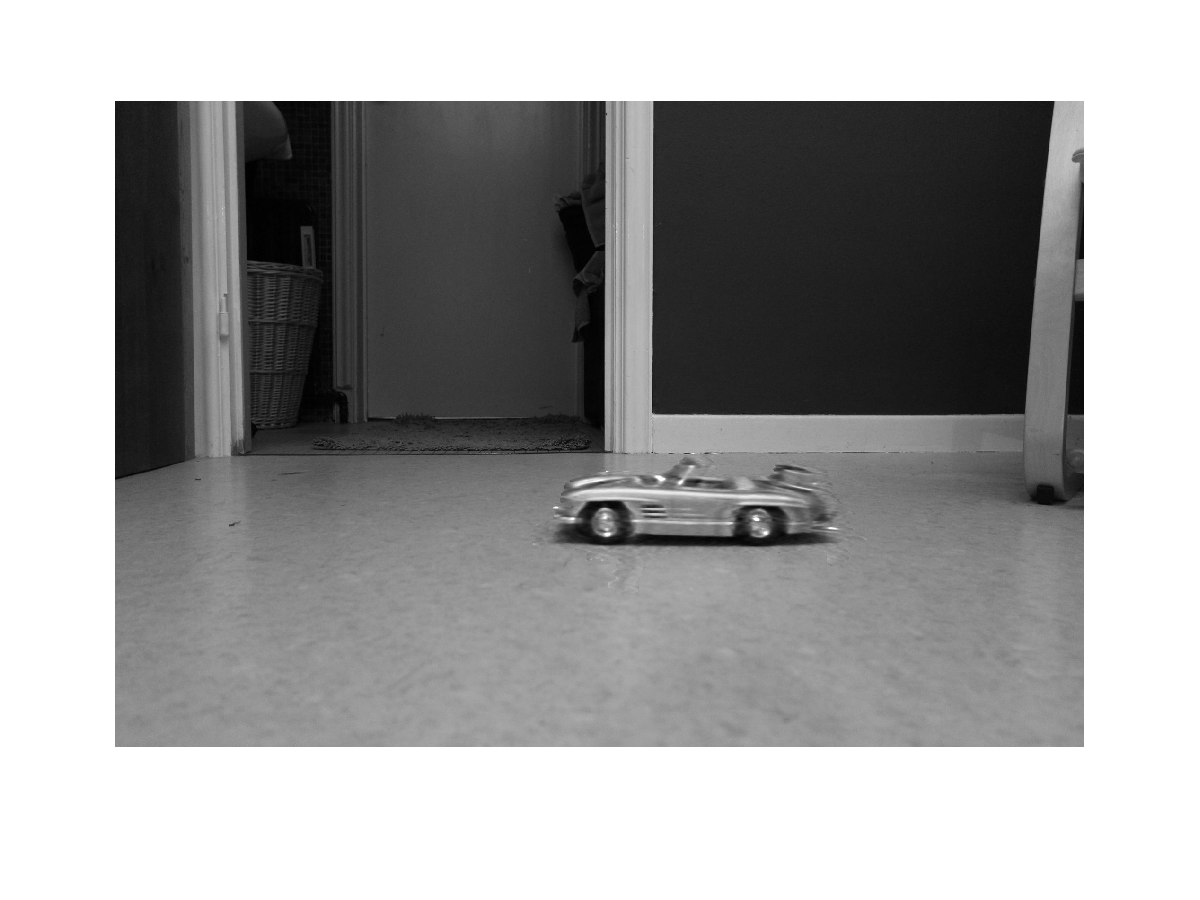
\includegraphics[trim=6cm 4cm 4cm 5cm,clip,width=\textwidth]{car1-5_1-20.png}
    \end{myfigsub}
    \begin{myfigsub}{car1-5_1-60}
      {``select-lucy'' with 60 iterations}{0.49}
      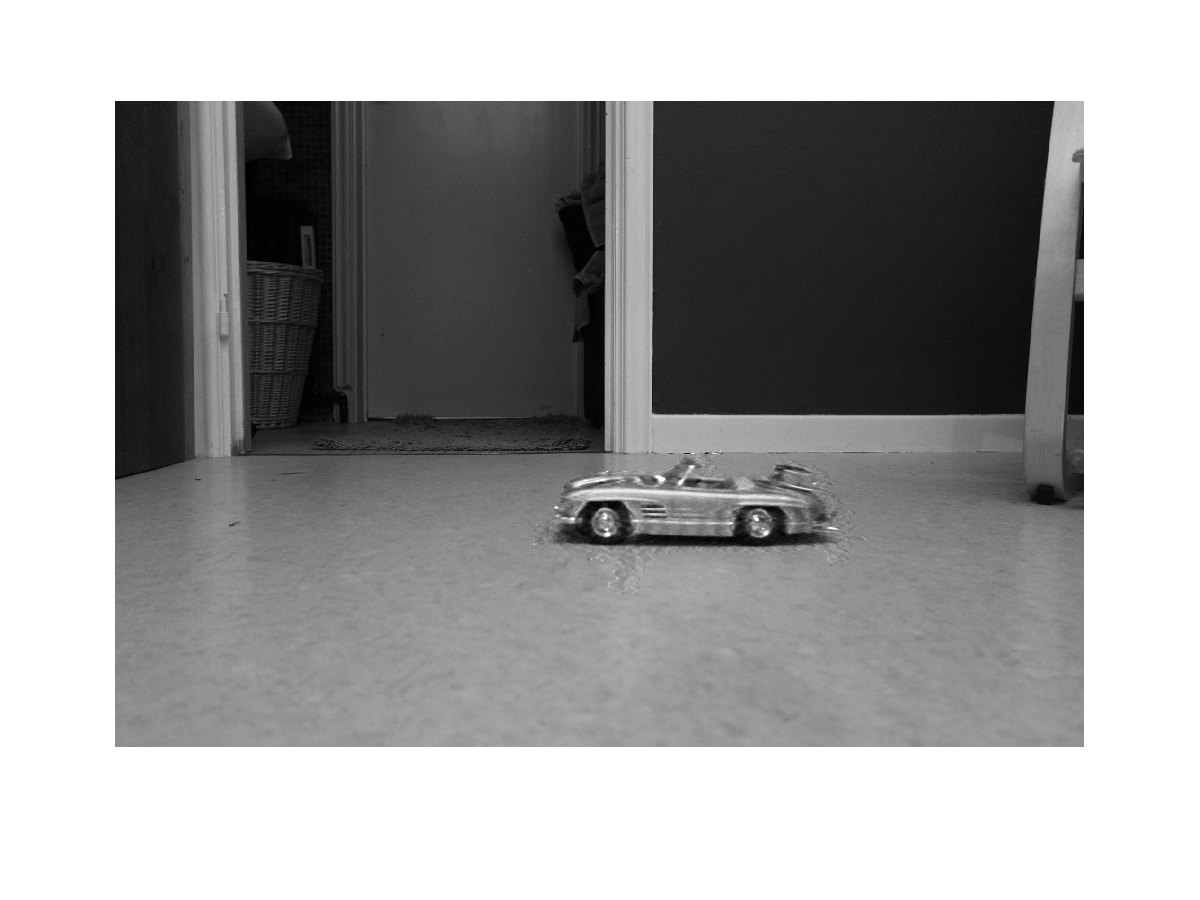
\includegraphics[trim=6cm 4cm 4cm 5cm,clip,width=\textwidth]{car1-5_1-60.png}
    \end{myfigsub}
    \begin{myfigsub}{car1-5_2-20}
      {``exact-lucy'' with 20 iterations}{0.49}
      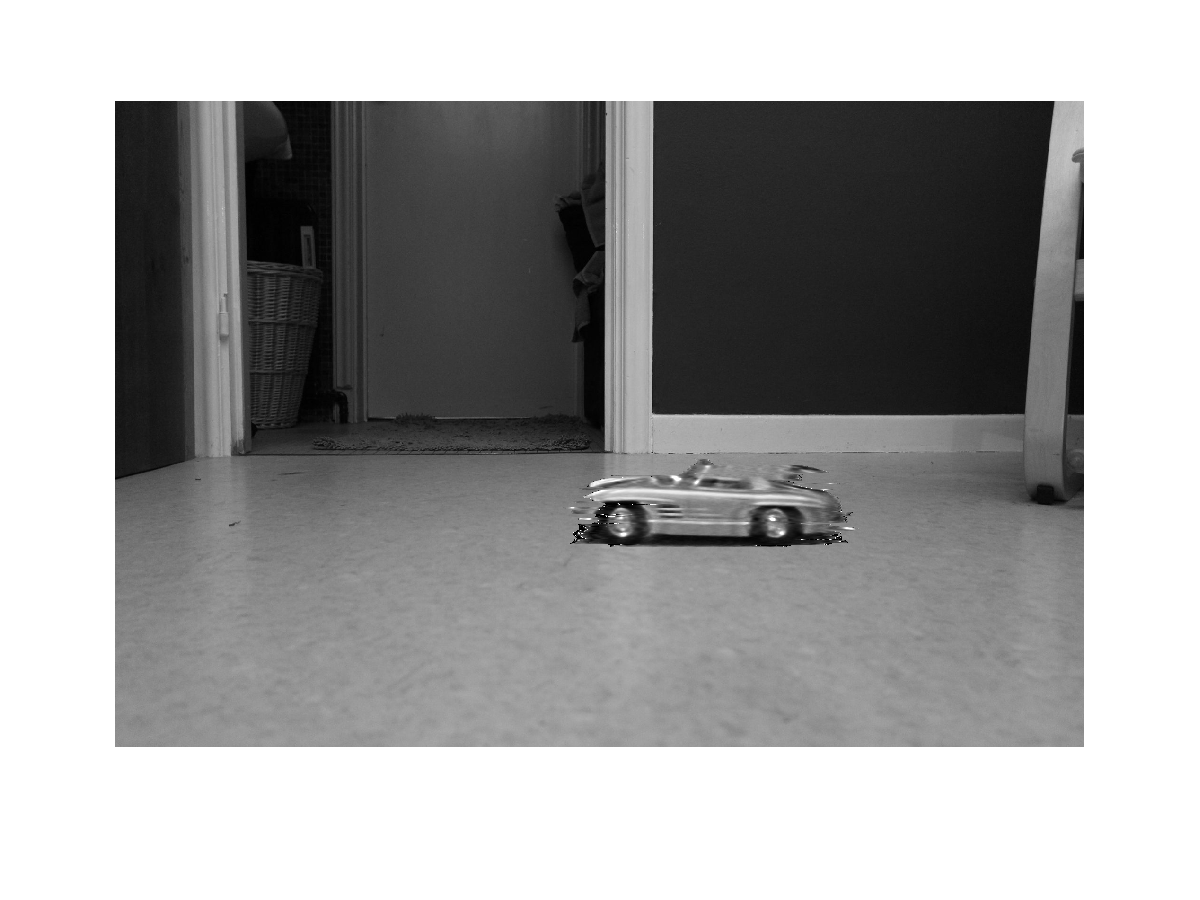
\includegraphics[trim=6cm 4cm 4cm 5cm,clip,width=\textwidth]{car1-5_2-20.png}
    \end{myfigsub}
    \begin{myfigsub}{car1-5_2-60}
      {``exact-lucy'' with 60 iterations}{0.49}
      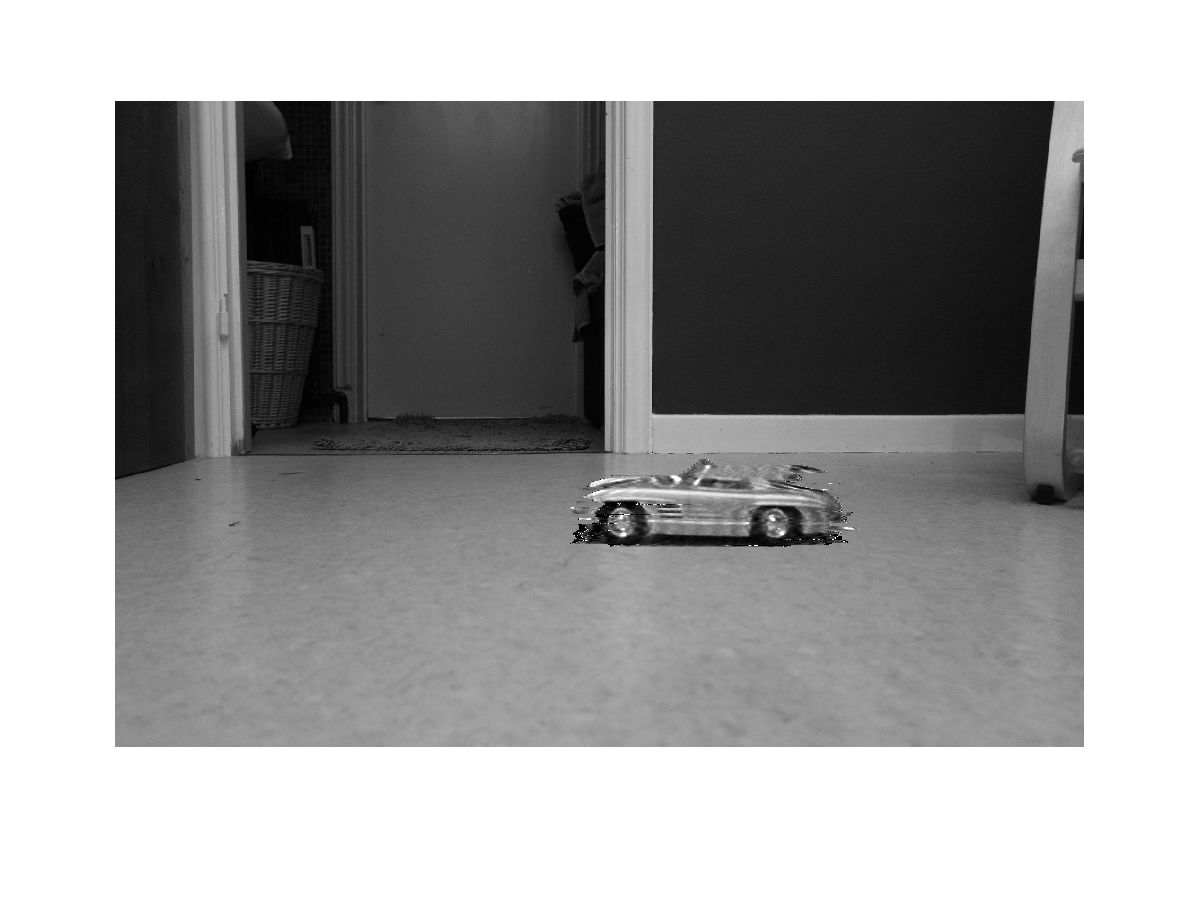
\includegraphics[trim=6cm 4cm 4cm 5cm,clip,width=\textwidth]{car1-5_2-60.png}
    \end{myfigsub}
    \begin{myfigsub}{car1-5_3}
      {Wiener}{0.49}
      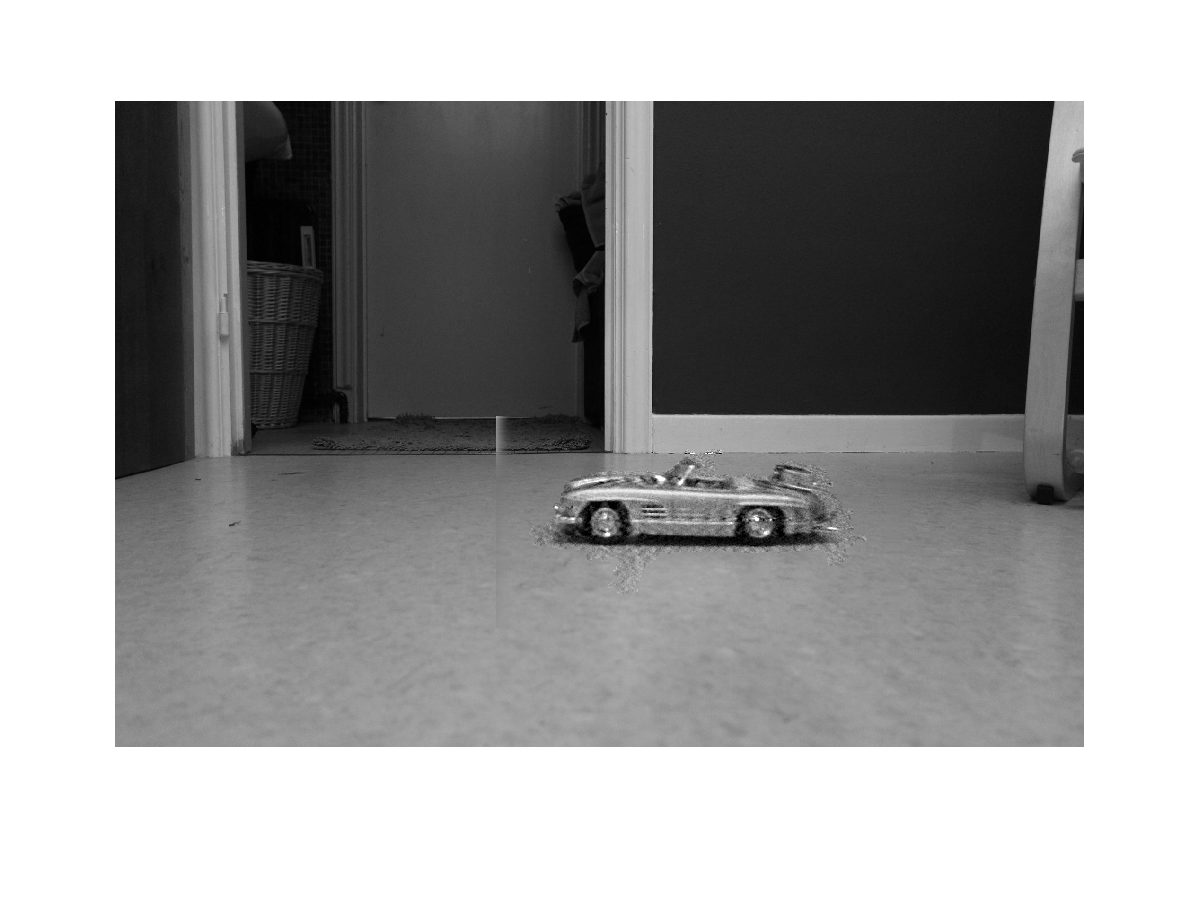
\includegraphics[trim=6cm 4cm 4cm 5cm,clip,width=\textwidth]{car1-5_3.png}
    \end{myfigsub}
    \begin{myfigsub}{car1}
      {Initial blurred image}{0.49}
      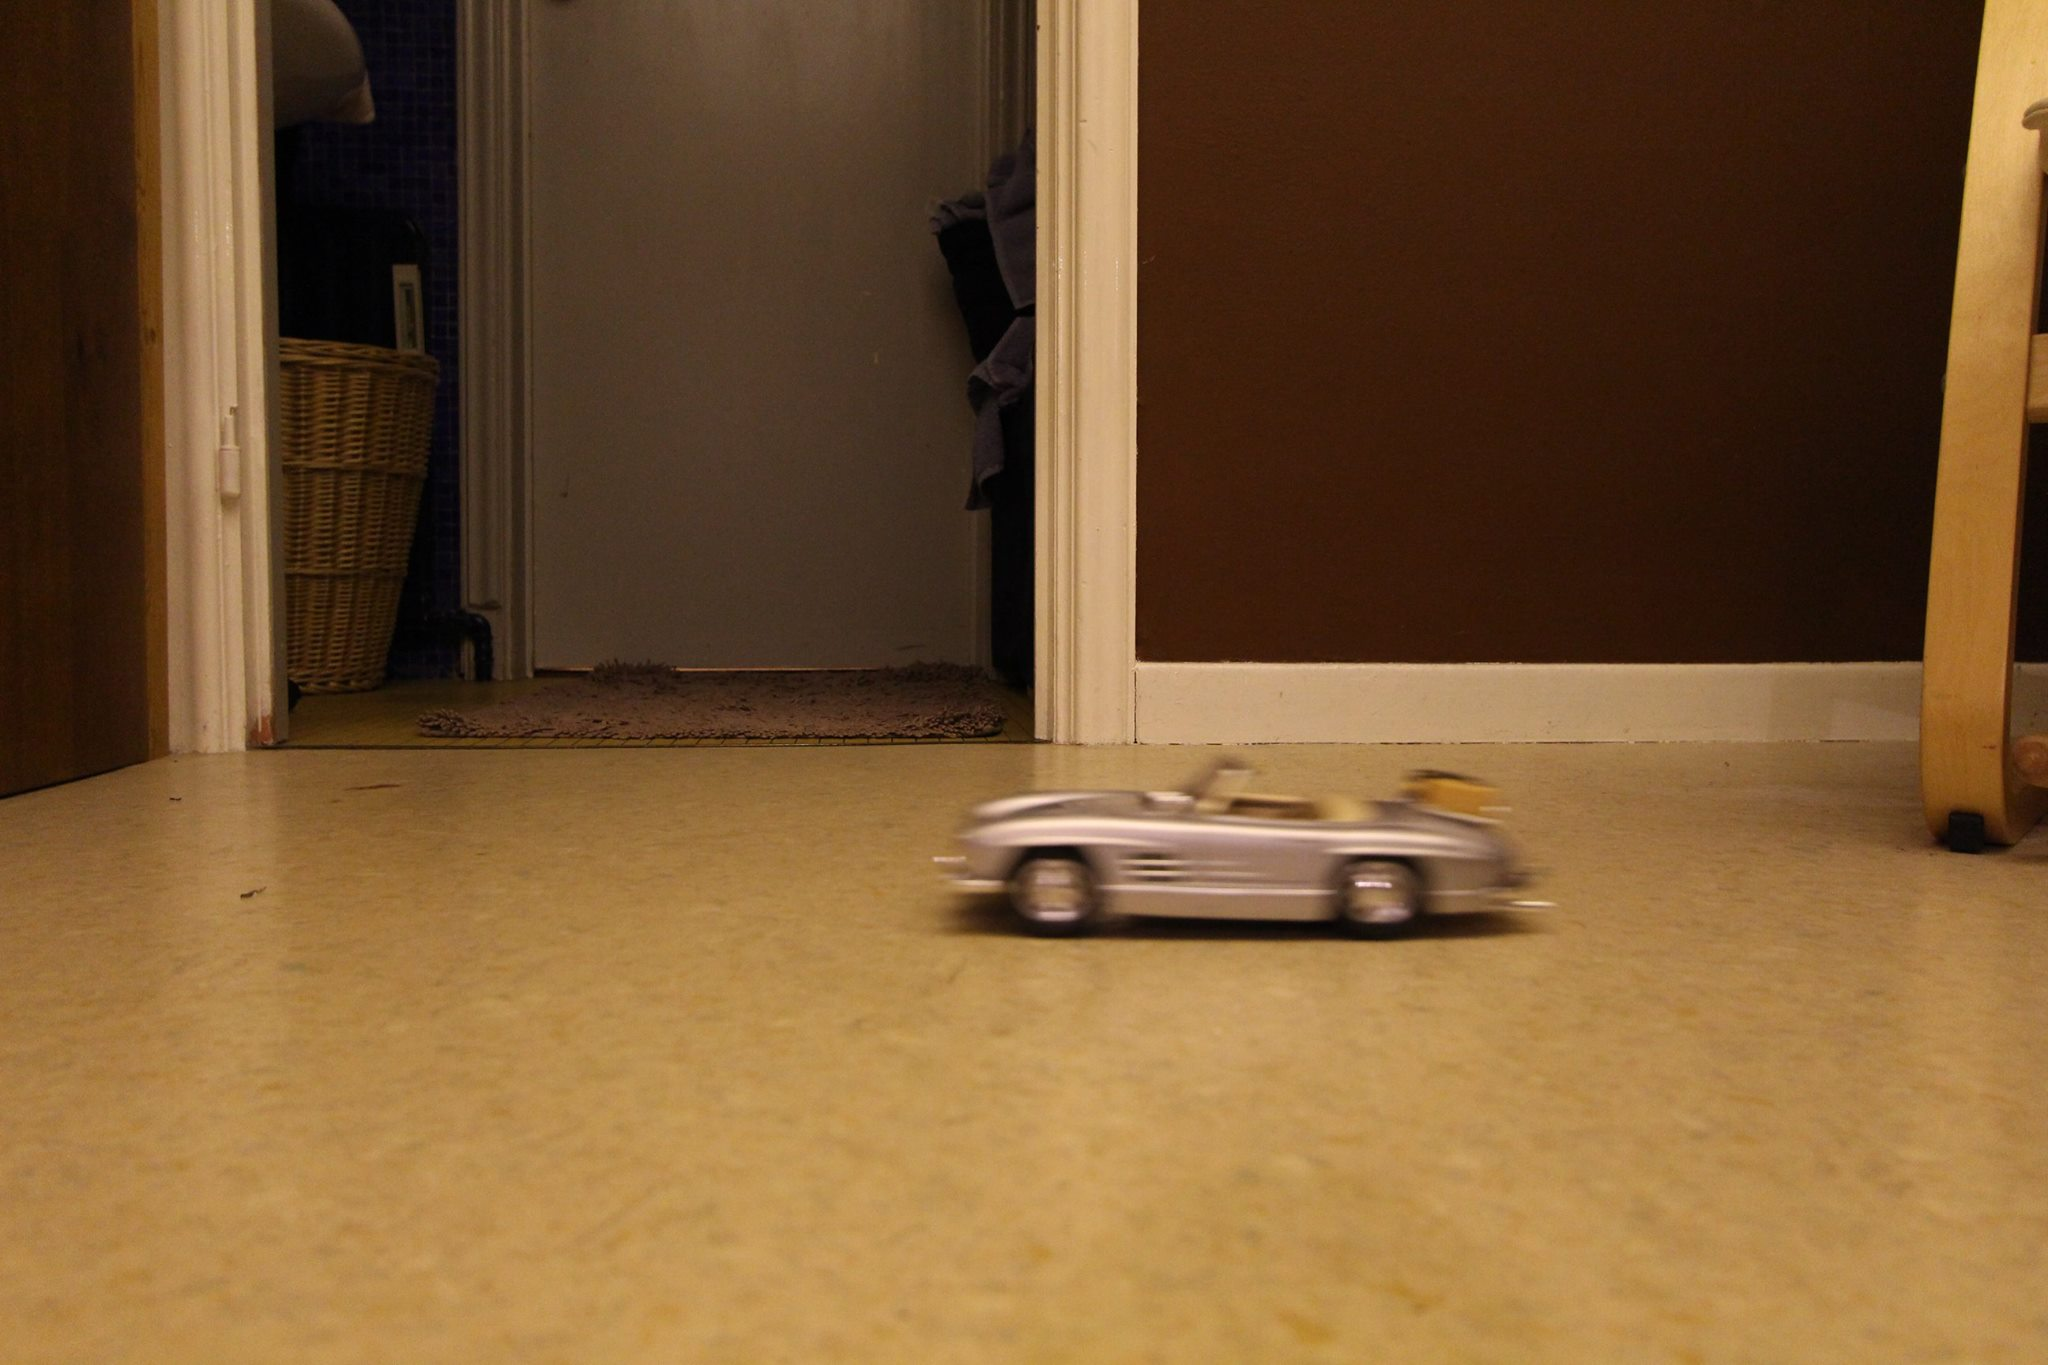
\includegraphics[trim=18cm 4.5cm 7cm 15cm,clip,width=\textwidth]{car1.jpg}
    \end{myfigsub}
  \end{myfig}
  \framebreak
  \begin{itemize}
    \item ``select-lucy'': Slow and borders effects but robust and precise.
    \item ``exact-lucy'': Slow and sensible to ``exact'' foreground estimation but precise and no border effect.
    \item ``wiener'': Fast but not sharp.
  \end{itemize}
\end{frame}
